\documentclass{article}
\usepackage[top=1.0in,bottom=1.0in,left=1.0in,right=1.0in]{geometry}
\usepackage{amsmath,amssymb,amsthm,amsfonts}
\usepackage[utf8]{inputenc}
\usepackage[T2A]{fontenc}
\usepackage[english,russian]{babel}
\usepackage{hyperref}
\usepackage{graphics,graphicx}

\title{Arcturus: эффективные доказательства для конфиденциальных транзакций}
\author{Саранг Ноезер (Sarang Noether) \\ Исследовательская лаборатория Monero (Monero Research Lab) \\ \texttt{sarang.noether@protonmail.com}}
\date{\today}

\newcommand{\F}{\mathbb{F}}
\newcommand{\N}{\mathbb{N}}
\newcommand{\hs}{\mathsf{H}}
\newcommand{\hp}{\mathcal{H}}
\newcommand{\com}{\operatorname{Com}}
\newcommand{\A}{\mathcal{A}}

\newcommand{\sumi}{\sum_{i=0}^{n-1}}
\newcommand{\sumj}{\sum_{j=0}^{m-1}}
\newcommand{\sumk}{\sum_{k=0}^{N-1}}
\newcommand{\sumu}{\sum_{u=0}^{w-1}}

\newtheorem{theorem}{Теорема}
\theoremstyle{definition}
\newtheorem{definition}{Определение}


\begin{document}

\maketitle


\begin{abstract}
В случае с распределёнными цифровыми активами конфиденциальные транзакции используются для демонстрации равенства значений, скрытых в обязательствах при сохранении неопределённости подписанта.
В прошлой работе было описано доказательство знания открытия обязательств по нулю с одинаковым индексом для всего множества наборов обязательств с сохранением неопределённости подписанта, а также оценка верифицируемой случайной функции, используемой в качестве связующего тега и использующей это с целью построения связываемой кольцевой подписи, под названием Triptych, которое может использоваться как структурный элемент модели конфиденциальных транзакций.
В данной работе нами предлагается расширение Triptych для построения Arcturus, системы доказательства, позволяющей доказать знание открытия множества обязательств по нулю в пределах одного набора, правильность структуры верифицируемой случайной функции, оцениваемой при каждом открытии, и равенство значений в отдельном списке обязательств в пределах одного доказательства. Несмотря на то, что надёжность зависит от нового допуска сложности двойного дискретного логарифма, мы используем данные, взятые из блокчейна Monero, чтобы продемонстрировать, что Arcturus может использоваться в рамках модели конфиденциальных транзакций с целью обеспечения более быстрой групповой верификации в сравнении с существующими на сегодня конструкциями без каких-либо доверенных настроек.
\end{abstract}


\section{Введение}
Распределённые цифровые активы, начиная с Bitcoin, при авторизации транзакций и передаче прав на трату средств используют кольцевые подписи.
Несмотря на то, что ранние протоколы, в основе которых лежит модель, предложенная Bitcoin, имеют преимущество, связанное с простотой, им не хватает необходимых свойств, обеспечивающих приватность и неотличимость транзакций. В частности, граф адресов и подписи, формируемый блокчейном для таких цифровых активов, очень просто отследить, а суммы, которые в соответствии с подписью разрешено переводить в транзакции, видимы.
Чтобы защитить пользователей распределённых активов и обеспечить более высокий уровень неотличимости транзакций в целях взаимозаменяемости, на пути к конфиденциальным транзакциям было предложено и реализовано несколько методов.

Протокол CryptoNote, его раннее предложение, связанное с сокрытием графов транзакций, полагается на связываемые кольцевые подписи в ключе выходов транзакций с обозначенными суммами \cite{cryptonote}; транзакция включает в себя отдельную подпись для каждой такой суммы, в результате чего возникают проблемы с масштабированием.

Другим усовершенствованием стал протокол RingCT \cite{ringct}, который использовал обязательства Педерсена по суммам, связанным с выходами транзакций, и расширял структуру кольцевой подписи, предложенную Лю и \text{др.} (Liu et al.) в работе \cite{liu}, так чтобы поддерживались параллельные подписи в матричном расположении, что устраняло необходимость в обозначенных выходах транзакций.
Тем не менее, обе эти конструкции используют связываемые кольцевые подписи, размер которых масштабируется линейно с размером анонимной группы, используемой для создания каждой подписи.
Более поздние методы обеспечения приватности транзакций используют аккумуляторы, чтобы представить заданное состояние выходов транзакций.
Zerocoin \cite{zerocoin} для подтверждения правильности транзакций задействовал аккумуляторы RSA и связанные доказательства, но суммы были фиксированными, протокол использовал очень большие и неэффективные доказательства, транзакции ограничивались простой операцией сжигания-создания монет в прозрачном блокчейне, а применение групп RSA требовало процесса доверенной настройки.
Другой, более поздней работой стал Zerocash \cite{zerocash}, который заменил аккумуляторы RSA и связанные доказательства более краткими доказательствами, относящимися к аккумуляторам дерева Меркла, позволяя совершать анонимные переводы с произвольными суммами.
Тем не менее, Zerocoin как и Zerocash использовал систему доказательства, требующую доверительной настройки; в конечном счёте это послужило основанием для протоколов Zcash.

До недавнего времени протоколы транзакций, целью которых являлось обеспечение устойчивого сокрытия подписанта, гибкой непосредственной анонимной передачи произвольных сумм, подразумевали некоторый компромисс между реализацией не требующей доверия структуры и эффективности с точки зрения размера доказательств и времени верификации.

Последняя работа в этой области опирается на одну из двух новых систем доказательства для построения транзакций, которая масштабируется логарифмически с размером указываемой доказывающей стороной анонимной группы, но при этом не требует доверенных настроек. Система доказательства, использующая одно из многих обязательств по нулю, предложенная Гротом и Кёльвейсом (Groth and Kohlweiss) в работе \cite{groth}, использовалась для построения простых кольцевых подписей и транзакций в стиле Zerocoin, а позднее была расширена Бутлем (Bootle) \cite{bootle} так, чтобы более эффективно поддерживать рассчитываемые кольцевые подписи.

Эта система доказательства формирует основу протокола Lelantus \cite{lelantus}, расширяющего модель транзакций в стиле Zerocoin, предложенную в работе \cite{groth}, за счёт использования обязательств Педерсена с множеством оснований, включающих в себя суммы наряду с порядковыми номерами; изменённые доказательства демонстрируют равенство, а множественные доказательства необходимы для создания типичных транзакций.

Тем не менее транзакции Lelantus позволяют идентифицировать отправителя транзакции позднее, когда получатель решит потратить их средства; внесение соответствующих исправлений решает проблему отслеживания, но это делается за счёт устранения полезной конструкции одноразовых адресов, гарантирующих анонимность получателя.

Та же система доказательства, что была описана в работе \cite{groth}, используется и в Triptych \cite{triptych}, а если точнее, это конструкция многомерной связываемой кольцевой подписи, которая может использоваться для построения конфиденциальных транзакций подобно тому, как это описано в работе \cite{ringct}; что важно, Triptych поддерживает одноразовые адреса и произвольные суммы, но при этом по-прежнему требует использования множества доказательств для траты множества выходов транзакций.

Что интересно, последняя независимая работа расширяет схему \cite{groth} так, чтобы поддерживались обязательства по множеству обязательств в одном списке (что мы также показываем ниже), что определённым образом применимо в отношении Zether \cite{zether}; тем не менее, в данном случае используется подход, отличающийся от того, что мы используем в данной работе, и, по-видимому, предполагающий больший размер доказательств.

Система доказательства Bulletproofs \cite{bulletproofs} использует метод сжатия скалярного произведения для построения доказательств диапазона и соответствия схемы с возможностью их логарифмического масштабирования.
Помимо большее широкого развёртывания доказательств диапазона обязательств, структура, лежащая в основе Bulletproofs, используется для построения более специализированных систем доказательства конфиденциальных транзакций.
Omniring \cite{omniring} использует этот метод для построения транзакций, демонстрирующих право на трату множества входов транзакций с сокрытием подписанта в рамках одного единственного доказательства, а доказательство диапазона при этом интегрируется напрямую. В результате получаются очень маленькие доказательства; тем не менее, если сравнивать с другими подходами, время верификации увеличивается, а требования к генерированию уникальной группы означают, что доказательства нельзя эффективно верифицировать группами.

RingCT 3.0 \cite{rct3} также использует структуру в стиле Bulletproofs.

В ранней версии транзакции требовали использования отдельных доказательств для множества входов; и, несмотря на то, что обновлённые версии уже позволяли использовать одно доказательство для всех входов транзакции, также требовалось, чтобы количество входов дополнялось и становилось больше в два раза, что повышало сложность верификации.


\subsection{Наш вклад}
Нами была расширена система доказательства Triptych, предложенная в работе \cite{triptych}, по двум важным направлениям, и полученная система была названа Arcturus.

Во-первых, мы даём доказывающей стороне возможность демонстрировать одновременное знание множества подписывающих ключей в рамках единственного доказательства, использующего один набор комбинированных элементов доказательства; в отличие от того, что предлагалось в работе \cite{rct3}, наше изменение допускает использование любого количества входов транзакции без каких-либо ограничений.

Мы сохраняем оценку верифицируемой случайной подписи, создающей связующие теги, необходимые для обнаружения повторного подписания с использованием того же открытия обязательства по доказательствам.

Во-вторых, мы демонстрируем равенство значения обязательства Педерсена напрямую в пределах того же доказательства; в частности, мы показываем, что определённая комбинация обязательств по входам и выходам суммируется в обязательство по нулю. Мы отмечаем, что надёжность полученной системы доказательства зависит от нового допуска сложности двойного дискретного логарифма. И, несмотря на то, что мы считаем использование этого нового допуска разумным, он ещё не тестировался.

В совокупности эти изменения могут найти применение в протоколе транзакций, обеспечивая эффективность конфиденциальных транзакций в блокчейне при отсутствии необходимости в доверенных настройках.

В рамках транзакции может быть подписано множество входов с сокрытием подписанта, а также может быть доказана сбалансированность транзакции при помощи единственного доказательства, что является главным усовершенствованием используемых в настоящее время конструкций, требующих множества доказательств и отдельных вспомогательных обязательств Педерсена по сумме.

Кроме того, нами используются фактические данные блокчейна Monero, цифрового актива, чтобы напрямую сравнить общий размер и время верификации Arcturus и Triptych, и двух отдельных конструкций RingCT 3.0. Нами было выявлено, что Arcturus обеспечивает превосходные показатели верификации, если сравнивать с другими конструкциями конфиденциальных транзакций, не требующих доверенных настроек, при сравнимых показателях по масштабированию с точки зрения размера.


\section{Предварительные данные}

\subsection{Публичные параметры}
Допустим, \begin{math}\mathbb{G}\end{math} является циклической группой, в которой задача дискретного логарифмирования является сложной, но $F$ является её полем скалярных величин.

Допустим, $\hs: \{0,1\}^* \to \F$ и $\hp: \{0,1\}^* \to$ \begin{math}\mathbb{G}\end{math} является криптографической хеш-функцией.

Допустим, $N = n^m$ является положительным целым числом, где $m > 1$ (в случае с нашей конструкцией мы используем $n = 2$).

Допустим, $G$, $H$, $U$ и любая точка в форме $G_i$ или $H_i$ (возможно, с множеством индексов) являются единообразно случайными генераторами \begin{math}\mathbb{G}\end{math}, отношение дискретных логарифмов друг к другу не известно. Следует отметить, что все такие генераторы могут быть получены при помощи случайных публичных параметров; например, использование соответствующей хеш-функции с разделением доменов может подойти.

Подразумевается, что все такие публичные параметры включают в себя строку глобальной ссылки, известную всем участникам; в частности, для удобочитаемости нами в целом исключается явная ссылка на публичные параметры в определениях алгоритма и хешей транскрипта Фиата-Шамира.


\subsection{Тензорное обязательство}
Допустим, $\com$ является схемой аддитивно гомоморфного обязательства, обеспечивающего совершенное сокрытие, и (по крайней мере) являющегося обязательным для вычисления.

В данной работе мы допускаем использование простого расширения схемы обязательства Педерсена: для $x,r \in \F$ определяем $\com(x,r) \equiv rG + xH$ как обязательство по значению $x$ со степенью случайности $r$.

Для трёхмерного тензора $f \equiv (f_{i,j,k}) \subset \F$ и скрывающего фактора $r \in \F$ определяем тензорное обязательство Педерсена
$$\com(f,r) \equiv rG + \sum_{i,j,k} f_{i,j,k} G_{i,j,k}$$
используя фиксированные независимые генераторы, как было описано выше.

Подразумевается, что операции по тензорам производятся покомпонентно, например, если $f \equiv (f_{i,j,k})$ и $g \equiv (g_{i,j,k})$ являются такими тензорами для $\F$, то $f + g \equiv (f_{i,j,k} + g_{i,j,k})$ и так далее.


\subsection{Другая система обозначений}
Для целых чисел или элементов поля $i,j$ дельта-символ Кронекера $\delta(i,j)$ будет равен $1$, если $i=j$ и $0$ в противном случае, если берётся выход из соответствующего набора.

Иногда мы используем нижний индекс в форме $i_j$, чтобы обозначить разряд $j$ для $i$, где разложение $i$ берётся по основанию $n$ с заполнением длинны $m$:
$$\sum_{j=0}^{m-1} i_j n^j = i$$
Такая система обозначений используется там, где может возникнуть путаница.


\subsection{Сигма-протоколы}
Для заданного отношения $\mathcal{R}$ сигма-протокол $\mathcal{R}$ будет интерактивным протоколом запроса-ответа между доказывающей стороной и верификатором, в рамках которого доказывающая сторона желает убедить верификатора в том, что ей известно свидетельство, соответствующее утверждению, содержащемуся в $\mathcal{R}$.

Сигма-протокол является полным, надёжным и подразумевает нулевое разглашение информации.

Эти определения хорошо известны, и найти их можно, например, в работе \cite{groth}.

По существу, эти свойства предполагают следующее:
\begin{itemize}
\item \textit{Абсолютная полнота}: В случае со свидетельством по утверждению, содержащемуся в $\mathcal{R}$, добросовестная доказывающая сторона всегда сможет убедить добросовестного верификатора в его достоверности.
\item \textit{Особая надёжность}: При наличии утверждения в $\mathcal{R}$ это означает, что если доказывающая сторона способна выдать транскрипты действительных доказательств в ответ на множество запросов верификатора, то из этих транскриптов также можно извлечь и свидетельство по такому утверждению.
\item \textit{Особое нулевое разглашение при наличии добросовестного верификатора}: При наличии утверждения и запроса известного верификатора можно произвести смоделированный транскрипт без знания соответствующего действительного свидетельства.
\end{itemize}
Сигма-протоколы можно сделать неинтерактивными, если заменить случайные запросы верификатора запросами транскриптов на основе хешей в соответствии с моделью случайного оракула; это называется эвристическим подходом Фиата-Шамира \cite{fiat}.


\subsection{Допуск сложности}
Нами даётся определение новому допуску криптографической сложности, используемому далее для того, чтобы продемонстрировать надёжность нашей конструкции.

\begin{definition}[Задача двойного дискретного логарифмирования]
\label{def:dual}
Допустим, \begin{math}\mathbb{G}\end{math} является группой, для которой задача дискретного логарифмирования является сложной, допустим, $\F$ является её полем скалярных величин.
Допустим, $n > 0$.
Рассмотрим следующую игру между запрашивающей стороной и игроком $\A$ с вероятностным полиномиальным временем:
\begin{itemize}
\item Запрашивающая сторона единообразно случайным образом выбирает значения $G,H \in$ \begin{math}\mathbb{G}\end{math} и отправляет оба эти значения $\A$.
\item $\A$ выбирает и отправляет обратно множества $\{G_i\}_{i=0}^{n-1},\{H_i\}_{i=0}^{n-1} \subset$ \begin{math}\mathbb{G}\end{math} запрашивающей стороне.
\item Запрашивающая сторона единообразно случайным образом выбирает множество $\{\mu^i\}_{i=0}^{n-1} \subset \F$ и отправляет его $\A$.
\item $\A$ выбирает и отправляет обратно множество $\{x_i\}_{i=0}^{n-1} \subset \F$ запрашивающей стороне.
\end{itemize}
Мы можем утверждать, что игрок $\A$ победил в игре $(n,\epsilon,t)$ с решением задачи двойного дискретного логарифмирования, если в течение времени, не превышающего значение $t$ и с вероятностью, равной, по крайней мере, $\epsilon$, действительными были следующие условия:
\begin{itemize}
\item $\sumi \mu^i \left( G_i - x_iG \right) = 0$
\item $\sumi \mu^i \left( H - x_iH_i \right) = 0$
\item Существовал такой индекс $0 \leq i < n$, что либо $x_iG \neq G_i$, либо $x_iH_i \neq H$.
\end{itemize}
\end{definition}


\section{Система доказательства}
Нами предлагается сигма-протокол для следующего отношения:
\begin{multline*}
\mathcal{R} \equiv \Bigg\{ \{M_i\}_{i=0}^{N-1},\{P_i\}_{i=0}^{N-1},\{J^{(u)}\}_{u=0}^{w-1},\{Q_j\}_{j=0}^{T-1} \subset \mathbb{G} \: ; \: \left( \{l^{(u)}\}_{u=0}^{w-1}, \{r^{(u)}\}_{u=0}^{w-1}, y \right) : \\
M_{l^{(u)}} = r^{(u)}G \; \forall \: u \in [0,w) \text{ and } r^{(u)}J^{(u)} = U \; \forall \: u \in [0,w) \text{ and } \sum_{u=0}^{w-1} P_{l^{(u)}} - \sum_{j=0}^{T-1} Q_j = yG \Bigg\}
\end{multline*}

Здесь охвачены элементы, необходимые для авторизации транзакции, о которых мы будем говорить далее; знание подписывающих ключей $\{r^{(u)}\}$ демонстрирует, что у доказывающей стороны есть право на подписание входов транзакции, а также, а знание секретного ключа $y$ к разнице обязательства по сумме показывает, что суммы транзакции сбалансированы.

Наконец, сравнение верифицируемой случайной функции, используемой для получения $\{J^{(u)}\}$, будет использоваться для предотвращения попыток подписания одним и тем же секретным ключом без раскрытия соответствующего публичного ключа, что важно с точки сокрытия подписанта и защиты от попыток двойной траты в пределах доказательств или между ними.

На рисунках \ref{fig:sigma} и \ref{fig:sigma2} показано взаимодействие доказывающей стороны и верификатора. Затем мы доказываем, что действия доказывающей стороны и верификатора составляют сигма-протокол, являющийся совершенно правильным, и что он обладает свойствами особой надёжности и особого нулевого разглашения при наличии добросовестного верификатора.

\begin{figure}[htbp]
\centering
\fbox{\begin{minipage}{0.95\textwidth}
$\underline{\mathcal{P}:}$
\begin{itemize}
\item Выбираем случайное $r_A \in \F$ и $\left\{a_{j,i}^{(u)}\right\}_{i=1,j,u=0}^{n-1,m-1,w-1} \subset \F$.
Задаём $$\{a_{j,0}^{(u)}\}_{j,u=0}^{m-1,w-1} \equiv -\sum_{i=1}^{n-1} a_{j,0}^{(u)}$$ и определяем $A \equiv \com(a,r_A)$.
\item Определяем $\left\{\sigma_{j,i}^{(u)}\right\}_{i,j,u=0}^{n-1,m-1,w-1} \subset \F$ так, чтобы $\sigma_{j,i}^{(u)} \equiv \delta\left(l_j^{(u)},i\right)$ (пользуясь нашим обозначением разложения) и выбираем случайное $r_B \in \F$.
Определяем $B \equiv \com(\sigma,r_B)$.
\item Выбираем случайное $r_C \in \F$ и определяем $C \equiv \com(a(1-2\sigma), r_C)$.
\item Выбираем случайное $r_D \in \F$ и определяем $D \equiv \com(-a^2, r_D)$.
\item Для $0 \leq u < w$ определяем такие коэффициенты $\left\{p_{k,j}^{(u)}\right\}_{k,j=0}^{N-1,m-1}$, чтобы $$p_k^{(u)}(x) \equiv \prod_{j=0}^{m-1} \left( \sigma_{j,k}^{(u)}x + a_{j,k}^{(u)} \right) = \delta\left(l^{(u)},k\right)x^m + \sumj p_{k,j}^{(u)}x^j$$ (пользуясь нашим обозначением разложения).
Затем определяем $p_{k,j} \equiv \sumu p_{k,j}^{(u)}$ и $p_k(x) \equiv \sumu p_k^{(u)}(x)$ соответственно.
\item Выбираем случайное $\left\{\rho_j\right\}_{j,u=0}^{m-1,w-1}, \left\{\overline{\rho}_j^{(u)}\right\}_{j,u=0}^{m-1,w-1} \subset \F$.
\item Задаём $\mu \equiv \hs(\{M_k\},\{P_k\},\{J^{(u)}\})$ (так же и для включения всех публичных параметров).
\item Определяем $\{X_j\}_{j=0}^{m-1} \subset $\begin{math}\mathbb{G}\end{math} так, чтобы $$X_j \equiv \sumk p_{k,j}\mu^kM_k + \sumu \rho_j^{(u)}G$$
\item Определяем $\{Y_j\}_{j=0}^{m-1} \subset $\begin{math}\mathbb{G}\end{math} так, чтобы $$Y_j \equiv U \sumk p_{k,j}\mu^k + \sumu \rho_j^{(u)}J^{(u)}$$
\item Определяем $\{Z_j\}_{j=0}^{m-1} \subset $\begin{math}\mathbb{G}\end{math} так, чтобы $$Z_j \equiv \sumk p_{k,j}P_k + \sumu \overline{\rho}_j^{(u)}G$$
\end{itemize}

$\underline{\mathcal{P} \to \mathcal{V}:}$ \\
$A,B,C,D,\{X_j\},\{Y_j\},\{Z_j\}$
\end{minipage}}
\caption{Сигма-протокол для $\mathcal{R}$}
\label{fig:sigma}
\end{figure}

\begin{figure}[htbp]
\centering
\fbox{\begin{minipage}{0.95\textwidth}
$\underline{\mathcal{V} \to \mathcal{P}:}$ \\
$\xi \in \{0,1\}^*$ \\

$\underline{\mathcal{P}(\xi):}$
\begin{itemize}
\item Определяем $\left\{f_{j,i}^{(u)}\right\}_{i=1,j,u=0}^{n-1,m-1,w-1}$ так, чтобы $f_{j,i}^{(u)} \equiv \sigma_{j,i}^{(u)}\xi + a_{j,i}^{(u)}$.
\item Определяем $z_A \equiv r_A + \xi r_B$ и $z_C \equiv \xi r_C + r_D$.
\item Определяем $\left\{z_R^{(u)}\right\}_{u=0}^{w-1} \subset \F$ так, чтобы $$z_R^{(u)} \equiv \mu^{l^{(u)}}r^{(u)}\xi^m - \sumj \rho_j^{(u)}\xi^j$$
\item Определяем: $$z_S \equiv \xi^m \left( \sumu s^{(u)} - \sum_{j=0}^{T-1} t_j \right) - \sumj \left( \xi^j \sumu \overline{\rho}_j^{(u)} \right)$$
\end{itemize}

$\underline{\mathcal{P} \to \mathcal{V}:}$ \\
$\{f_{j,i}^{(u)}\}_{j=0,i=1,u=0}^{m-1,n-1,w-1},z_A,z_C,\{z_R^{(u)}\},z_S$ \\

$\underline{\mathcal{V}:}$
\begin{itemize}
\item Для $0 \leq u < w$ и $0 \leq j < m$ задаём: $$f_{j,0}^{(u)} \equiv \xi - \sum_{i=1}^{n-1} f_{j,i}^{(u)}$$
\item Принимаем результат исключительно в том случае, если:
\begin{eqnarray}
A + \xi B &=& \com(f,z_A) \label{eqn:ab} \\
\xi C + D &=& \com(f(\xi-f),z_C) \label{eqn:cd} \\
\sumk \mu^kM_k \left[ \sumu \left( \prod_{j=0}^{m-1} f_{j,k_j}^{(u)} \right) \right] - \sumj \xi^jX_j - \sumu z_R^{(u)}G &=& 0 \label{eqn:x} \\
U \sumk \mu^k \left[ \sumu \left( \prod_{j=0}^{m-1} f_{j,k_j}^{(u)} \right) \right] - \sumj \xi^jY_j - \sumu z_R^{(u)}J^{(u)} &=& 0 \label{eqn:y} \\
\sumk P_k \left[ \sumu \left( \prod_{j=0}^{m-1} f_{j,k_j}^{(u)} \right) \right] - \sumj \xi^jZ_j - \xi^m\sum_{j=0}^{T-1} Q_j - z_SG &=& 0 \label{eqn:z}
\end{eqnarray}
\end{itemize}
\end{minipage}}
\caption{Сигма-протокол для $\mathcal{R}$ (продолжение)}
\label{fig:sigma2}
\end{figure}


\section{Безопасность}
\begin{theorem}
Сигма-протокол, представленный на рисунках\ref{fig:sigma} и \ref{fig:sigma2}, отражает отношение $\mathcal{R}$ и является совершенно правильным, обладает свойствами особой надёжности $(m+1)$ и особого нулевого разглашения при наличии добросовестного верификатора.
\end{theorem}

\begin{proof}
Доказательство подобно тому, что приводится в работе \cite{triptych} и которое, в свою очередь, следует методам, описанным в работах \cite{groth,bootle}.

Чтобы показать, что протокол является абсолютно полным, предположим, что верификатор получает честное доказательство. Нам необходимо продемонстрировать, что все уравнения верификатора выполняются.

Чтобы показать, что уравнение \ref{eqn:ab} выполняется, отмечаем, что поскольку
\begin{eqnarray*}
A + \xi B &=& \com(a + \xi\sigma,r_A + \xi r_B) \\
&=& \com(a + \xi\sigma,z_A),
\end{eqnarray*}
достаточно продемонстрировать, что $f_{j,i}^{(u)} = a_{j,i}^{(u)} + \xi\sigma_{j,i}^{(u)}$ для всех $0 \leq i < n$ и $0 \leq j < m$, и $0 \leq u < w$.
Если $i \neq 0$, значит, данное уравнение выполняется по определению $f_{j,i}^{(u)}$.
В случае если $i = 0$ всё будет иначе.
Чтобы показать это, воспользуемся тем фактом, что $$\sumi \sigma_{j,i}^{(u)} = 1$$ для всех $0 \leq j < m$ и $0 \leq u < w$, в соответствии с конструкцией:
\begin{eqnarray*}
f_{j,0}^{(u)} &=& \xi - \sum_{i=1}^{n-1} f_{j,i}^{(u)} \\
&=& \xi - \sum_{i=1}^{n-1} \left( a_{j,i}^{(u)} + \xi\sigma_{j,i}^{(u)} \right) \\
&=& \xi - \sum_{i=1}^{n-1} a_{j,i}^{(u)} - \xi\sum_{i=1}^{n-1} \sigma_{j,i}^{(u)} \\
&=& \xi + a_{j,0}^{(u)} - \xi\left( 1 - \sigma_{j,0}^{(u)} \right) \\
&=& a_{j,0}^{(u)} + \xi\sigma_{j,0}^{(u)}
\end{eqnarray*}

Мы демонстрируем, что уравнение \ref{eqn:cd} выполняется.
Так как:
\begin{eqnarray*}
\xi C + D &=& \com(\xi a(1 - 2\sigma) - a^2,\xi r_C + r_D) \\
&=& \com(\xi a(1 - 2\sigma) - a^2,z_C),
\end{eqnarray*}
достаточно показать, что $$f_{j,i}^{(u)}\left( \xi - f_{j,i}^{(u)} \right) = \xi a_{j,i}^{(u)}\left( 1 - 2\sigma_{j,i}^{(u)} \right) - \left(a_{j,i}^{(u)}\right)^2$$ для всех $0 \leq i < n$ и $0 \leq j < m$ и $0 \leq u < w$.
Мы используем нашу предшествующую работу и тот факт, что $\left(\sigma_{j,i}^{(u)}\right)^2 = \sigma_{j,i}^{(u)}$, поскольку $\sigma_{j,i}^{(u)} \in \{0,1\}$:
\begin{eqnarray*}
f_{j,i}^{(u)}\left( \xi - f_{j,i}^{(u)} \right) &=& \left( a_{j,i}^{(u)} + \xi\sigma_{j,i}^{(u)} \right)\left( \xi - a_{j,i}^{(u)} - \xi\sigma_{j,i}^{(u)} \right) \\
&=& a_{j,i}^{(u)}\xi - \left(a_{j,i}^{(u)}\right)^2 - 2a_{j,i}^{(u)}\xi\sigma_{j,i}^{(u)} + \left( \xi^2\sigma_{j,i}^{(u)} - \xi^2\left(\sigma_{j,i}^{(u)}\right)^2 \right) \\
&=& a_{j,i}^{(u)}\xi - \left(a_{j,i}^{(u)}\right)^2 - 2a_{j,i}^{(u)}\xi\sigma_{j,i}^{(u)} + \left( \xi^2\left(\sigma_{j,i}^{(u)}\right)^2 - \xi^2\left(\sigma_{j,i}^{(u)}\right)^2 \right) \\
&=& \xi a_{j,i}^{(u)}\left( 1 - 2\sigma_{j,i}^{(u)} \right) - \left(a_{j,i}^{(u)}\right)^2
\end{eqnarray*}

Затем мы демонстрируем, что уравнение \ref{eqn:x} выполняется:
\begin{eqnarray*}
&& \sumk \mu^kM_k \left[ \sumu \left( \prod_{j=0}^{m-1} f^{(u)}_{j,k_j} \right) \right] - \sumj \xi^jX_j - \sumu z^{(u)}_RG \\
&=& \sumk \mu^kM_k p_k(\xi) - \sumj \xi^j \left( \sumk p_{k,j}\mu^kM_k + \sumu \rho^{(u)}_jG \right) - \sumu z^{(u)}_RG \\
&=& \sumk \mu^kM_k \left( p_k(\xi) - \sumj \xi^j p_{k,j} \right) - \sumj \xi^j \sumu \rho^{(u)}_jG - \sumu z^{(u)}_RG \\
&=& \sumk \mu^kM_k \left[ \xi^m \sumu \delta\left( l^{(u)},k \right) \right] - \sumj \xi^j \sumu \rho^{(u)}_jG - \sumu\left[ \mu^{l^{(u)}}r^{(u)}\xi^m - \sumj \rho^{(u)}_j\xi^j \right]G \\
&=& \xi^m\sumu \mu^{l^{(u)}}r^{(u)}G - \sumj \xi^j \sumu \rho^{(u)}_jG - \xi^m\sumu \mu^{l^{(u)}}r^{(u)}G + \sumj \xi^j \sumu \rho^{(u)}_jG \\
&=& 0
\end{eqnarray*}

Уравнение \ref{eqn:y} выполняется с использованием той же алгебры:
\begin{eqnarray*}
&& \sumk \mu^kU \left[ \sumu \left( \prod_{j=0}^{m-1} f^{(u)}_{j,k_j} \right) \right] - \sumj \xi^jY_j - \sumu z^{(u)}_RJ^{(u)} \\
&=& \sumk \mu^kU p_k(\xi) - \sumj \xi^j \left( \sumk p_{k,j}\mu^kU + \sumu \rho^{(u)}_jJ^{(u)} \right) - \sumu z^{(u)}_RJ^{(u)} \\
&=& \sumk \mu^kU \left( p_k(\xi) - \sumj \xi^j p_{k,j} \right) - \sumj \xi^j \sumu \rho^{(u)}_jJ^{(u)} - \sumu z^{(u)}_RJ^{(u)} \\
&=& \sumk \mu^kU \left[ \xi^m \sumu \delta\left( l^{(u)},k \right) \right] - \sumj \xi^j \sumu \rho^{(u)}_j(r^{(u)})^{-1}U - \sumu\left[ \mu^{l^{(u)}}r^{(u)}\xi^m - \sumj \rho^{(u)}_j\xi^j \right](r^{(u)})^{-1}U \\
&=& x^m\sumu \mu^{l^{(u)}}U - \sumj \xi^j \sumu \rho^{(u)}_j(r^{(u)})^{-1}U - \xi^m\sumu \mu^{l^{(u)}}U + \sumj \xi^j \sumu \rho^{(u)}_j(r^{(u)})^{-1}U \\
&=& 0
\end{eqnarray*}

Наконец мы показываем, что выполняется уравнение \ref{eqn:z}:
\begin{eqnarray*}
&& \sumk P_k \left[ \sumu \left( \prod_{j=0}^{m-1} f^{(u)}_{j,k_j} \right) \right] - \sumj \xi^jZ_j - \xi^m\sum_{j=0}^{T-1} Q_j - z_SG \\
&=& \sumk P_k p_k(\xi) - \sumj \xi^j \left( \sumk p_{k,j}P_k + \sumu \overline{\rho}^{(u)}_jG \right) - \xi^m\sum_{j=0}^{T-1} Q_j - z_SG \\
&=& \sumk P_k \left( p_k(\xi) - \sumj \xi^j p_{k,j} \right) - \sumj \xi^j \sumu \overline{\rho}^{(u)}_jG - \xi^m\sum_{j=0}^{T-1} Q_j - z_SG \\
&=& \xi^m\sumu (s^{(u)}G + a_uH) - \sumj \xi^j \sumu \overline{\rho}^{(u)}_jG - \xi^m\sum_{j=0}^{T-1} (t_jG + b_jH) - \xi^m\left( \sumu s^{(u)} - \sum_{j=0}^{T-1} t_j \right)G + \\
&& \sumj \xi^j \sumu \overline{\rho}^{(u)}_jG \\
&=& \left( \sumu a_u - \sum_{j=0}^{T-1} b_j \right)H \\
&=& 0
\end{eqnarray*}
Следовательно, протокол является совершенно полным.

Затем мы демонстрируем, что сигма-протокол обладает свойством особого нулевого разглашения при наличии добросовестного верификатора.
Для этого мы строим симулятор, который при заданном запросе случайного верификатора $\xi$, может построить транскрипт доказательства с идентифчным распределением по действительному доказательству.

Сначала отмечаем, что симулятор, представленный в доказательстве Леммы 1 в работе \cite{bootle}, переводится практически так же, как в нашем случае, так как мы можем преобразовать тензорные обязательства в матричную структуру с необходимым свойством суммы.
Сначала единообразно случайным образом симулятор выбирает $B \in$ \begin{math}\mathbb{G}\end{math}; затем упомянутая лемма гарантирует действительное моделирование элементов доказательства $A,C,D,z_A,z_C,\{f^{(u)}_{j,i \neq 0}\}$, и на этой основе мы можем вычислить $\{f^{(u)}_{j,0}\}$.
В действительном доказательстве $B$ так же единообразно распределяется.

Элементы доказательства $\{X_j\}_{j=1}^{m-1},\{Y_j\}_{j=1}^{m-1}, \{Z_j\}_{j=1}^{m-1}$ являются независимыми и единообразно распределяются в действительном доказательстве, так как элементы $\{\rho_j\},\{\overline{\rho}_j\}$ распределяются единообразно, а задача дискретного логарифмирования в \begin{math}\mathbb{G}\end{math} является сложной; следовательно, симулятор выбирает их единообразно случайным образом.
Поскольку верификация требует, чтобы значения $X_0,Y_0,Z_0$ уникально определялись другими элементами в соответствующих множествах, они выбираются симулятором именно таким образом.

Наконец элементы $\{z^{(u)}_R\}_{u=0}^{w-1}$ и $z_S$ являются независимыми и единообразно распределяются в действительном доказательстве при наличии запроса случайного верификатора $\xi$, поэтому симулятор может выбирать их единообразно случайным образом.
Следовательно, протокол обладает свойством  особого нулевого разглашения при наличии добросовестного верификатора.

Мы утверждаем, что протокол обладает свойством особой надёжности $(m+1)$ при $m > 1$.
Чтобы продемонстрировать это, мы строим экстрактор, который при наличии $m+1$ действительных ответов на $m+1$ отдельных запросов верификатора по одному и тому же начальному утверждению производит действительное свидетельство для данного утверждения.
В частности, мы производим изменённое свидетельство для следующего отношения на базе информации, представленной в алгоритме доказывающей стороны, где $\mu$ определяется, как и раньше:
\begin{multline*}
\mathcal{R}' \equiv \Bigg\{ \{M_k\}_{k=0}^{N-1},\{P_k\}_{k=0}^{N-1},\{J^{(u)}\}_{u=0}^{w-1},\{Q_j\}_{j=0}^{T-1} \subset \mathbb{G} \: ; \: \left( \{l^{(u)}\}_{u=0}^{w-1}, \{r^{(u)}\}_{u=0}^{w-1}, y \right) : \\
\sumu \mu^{l^{(u)}} M_{l^{(u)}} = \sumu \mu^{l^{(u)}} r^{(u)}G \text{ and } \sumu \mu^{l^{(u)}} r^{(u)}J^{(u)} = \sumu \mu^{l^{(u)}} U \text{ and } \sum_{u=0}^{w-1} P_{l^{(u)}} - \sum_{j=0}^{T-1} Q_j = yG \Bigg\}
\end{multline*}
Отмечаем, что в том случае, если мы допускаем, что задача двойного дискретного логарифмирования в \begin{math}\mathbb{G}\end{math} является сложной, а $\hs$ смоделировано как случайный оракул, свидетельство для $\mathcal{R}'$, созданное экстрактором, также должно являться свидетельством для $\mathcal{R}$, использующим то же утверждение.
Это означает, что выделение свидетельства для $\mathcal{R}'$ является достаточным для обеспечения желаемой надёжности.

Предположим, что для данного утверждения у нас имеется множество $(m+1)$ отдельных запросов верификатора $\{\xi_e\}_{e=0}^m$, соответствующих отдельным действительным ответам следующей формы:
$$\left\{ \{{}_ef^{(u)}_{j,i}\}, \{{}_ez^{(u)}_R\}, {}_ez_S \right\}_{e=0}^m$$
В соответствии со свойством $3$-особой надёжности, описанным в работе \cite{bootle}, и при $m > 1$ мы получаем действительные выделения $\{\sigma^{(u)}_{j,i}\}_{u=0}^{w-1}$ и $\{a^{(u)}_{j,i}\}_{u=0}^{w-1}$, а свойство обязательства Педерсена гарантирует, что (с высокой степенью вероятности) мы получим:
$${}_ef^{(u)}_{j,i} = \sigma^{(u)}_{j,i}\xi_e + a^{(u)}_{j,i} \; \forall \: e \in [0,m]$$
При помощи выделенных значений вычисляем полином:
$$p_k(x) \equiv \sum_{u=0}^{w-1}\left[ \prod_{j=0}^{m-1} \left( \sigma^{(u)}_{j,k}x + a^{(u)}_{j,k} \right) \right]$$
для всех $k \in [0,N)$.
В результате выделения $\{\sigma^{(u)}_{j,i}\}_{u=0}^{w-1}$ получаем множество подписывающего индекса $\{l^{(u)}\}_{u=0}^{w-1}$.

Мы видим, что $p_k$ имеет степень $m$ только если $k \in \{l^{(u)}\}_{u=0}^{w-1}$.
Следовательно, существуют такие множества коэффициентов $\{\overline{X}_j,\overline{Y}_j,\overline{Z}_j\}_{j=0}^{m-1}$, уникально вычисленные на основе утверждения и выделенных значений, что уравнения \ref{eqn:x}, \ref{eqn:y} и \ref{eqn:z} имеют следующую форму:
\begin{eqnarray*}
\xi^m \sumu \mu^{l^{(u)}}M_{l^{(u)}} + \sumj \xi^j\overline{X}_j &=& \left( \sumu z^{(u)}_R \right)G \\
\xi^m \sumu \mu^{l^{(u)}}U + \sumj \xi^j\overline{Y}_j &=& \sumu z^{(u)}_RJ^{(u)} \\
\xi^m \sumu P_{l^{(u)}} + \sumj \xi^j\overline{Z}_j - \xi^m \sum_{j=0}^{T-1} Q_j &=& z_SG
\end{eqnarray*}

Строим матрицу Вандеромонда $V$, где ряд $e$ является вектором $(1,\xi_e,\ldots,\xi^m_e)$.
Поскольку все $\xi_e$ являются отдельными, ряды $V$ охватывают $\F^{m+1}$; следовательно, существуют такие взвешенные значения $\{\theta_e\}_{e=0}^m$, что полученная линейная комбинация рядов даёт вектор $(0,\ldots,0,1)$.
То есть $\sum_{e=0}^m \theta_e\xi_e^j = \delta(j,m)$.

Для каждого из предшествующих трёх уравнений, следовательно, мы можем построить линейную комбинацию по $e$. Для первого уравнения:
$$\sumu \mu^{l^{(u)}} M_{l^{(u)}} = \sum_{e=0}^m \theta_e\xi_e^m \left( \sumu \mu^{l^{(u)}} M_{l^{(u)}} \right) + \sum_{e=0}^m \theta_e \left( \sumj \xi_e^j \overline{X}_j \right) = \sumu \left( \sum_{e=0}^m \theta_e {}_ez^{(u)}_R \right) G$$
Следовательно, мы можем определить выделенные значения для каждого $r^{(u)}$:
$$r^{(u)} \equiv \frac{1}{\mu^{l^{(u)}}} \sum_{e=0}^m \theta_e {}_ez^{(u)}_R$$
Отмечаем, что то же самое свидетельство появляется во втором уравнении:
$$\sumu \mu^{l^{(u)}} U = \sum_{e=0}^m \theta_e\xi_e^m \left( \sumu \mu^{l^{(u)}} U \right) + \sum_{e=0}^m \theta_e \left( \sumj \xi_e^j \overline{Y}_j \right) = \sumu \left( \sum_{e=0}^m \theta_e {}_ez^{(u)}_R \right) J^{(u)}$$
Это означает, что требования к каждому $r^{(u)}$ соблюдены. То же действительно для третьего уравнения:
$$\sumu P_{l^{(u)}} - \sum_{j=0}^{T-1} Q_j = \sum_{e=0}^m \theta_e\xi_e^m \left( \sumu P_{l^{(u)}} - \sum_{j=0}^{T-1} Q_j \right) + \sum_{e=0}^m \theta_e \left( \sumj \xi_e^j \overline{Z}_j \right) = \left( \sum_{e=0}^m \theta_e {}_ez_S  \right)G$$
Следовательно, мы получаем $y \equiv \sum_{e=0}^m \theta_e {}_ez_S$.
\end{proof}


\section{Модель транзакций}
Теперь опишем, как сигма-протокол в $\mathcal{R}$ применяется в рамках модели конфиденциальных транзакций. Согласно данной модели транзакция использует так называемые \textit{выходы}, которые были сгенерированы при создании прошлых транзакций, и создаёт выходы для последующих транзакций.
Примечательно, что в случае с моделью \textit{конфиденциальных} транзакций мы хотим скрыть, какие входы транзакций используются, равно как и их соответствующие значения.

Выходы строятся как обязательства Педерсена по нулю таким образом, что публичный ключ выхода имеет форму $M \equiv rG$ где $r$ является подписывающим ключом.
Здесь нами не рассматривается метод создания ключей выходов, но подразумевается, что это происходим в другой части модели транзакций.
Каждый выход имеет обязательство по значению $P \equiv sG + aH$, где $a$ является суммой, а $s$ фактором обязательства.

Пользователь протокола формирует анонимную группу $\{M_i\}_{i=0}^{N-1}$, состоящую из выходов, взятых из предшествующих транзакций.
Отталкиваясь от этого, предположим, что множество $\{l^{(u)}\}_{u=0}^{w-1}$ представляет индексы $w$ выходов, по которым пользователь хочет подписаться; то есть пользователю известно такое $\{r^{(u)}\}_{u=0}^{w-1}$, что $r^{(u)}G = M_{l^{(u)}}$ для всех $0 \leq u < w$.
Для того чтобы поспособствовать сокрытию подписывающих индексов, предположим, что пользователь перемешал анонимную группу.
Каждый элемент анонимной группы имеет соответствующее обязательство по значению $\{P_i \equiv s_iG + a_iH\}_{i=0}^{N-1}$.

Далее, пользователь генерирует множество новых выходов, которые создаются при проведении транзакции, с соответствующими обязательствами по значению в форме $\{Q_j \equiv t_jG + b_jH\}_{j=0}^{T-1}$.
Так как значения в транзакции должны быть сбалансированы, должно соблюдаться следующее условие: $$\sum_{u=0}^{w-1} a_{l^{(u)}} = \sum_{j=0}^{T-1} b_j$$
Следует отметить, что для выходов, генерируемых при проведении транзакции, нет никакой анонимной группы.

Это используется для создания последовательность значений утверждения для отношения $\mathcal{R}$:
$$\left( \{M_i\}_{i=0}^{N-1}, \{P_i\}_{i=0}^{N-1}, \{(r^{(u)})^{-1}U\}_{u=0}^{w-1}, \{Q_j\}_{j=0}^{T-1} \: ; \: \left( \{l^{(u)}\}_{u=0}^{w-1}, \{r^{(u)}\}_{u=0}^{w-1}, \sumu a_{l^{(u)}} - \sum_{j=0}^{T-1} b_j \right) \right)$$
Пользователь генерирует доказательство, подтверждающее правильность этого утверждения, используя соответствующие секретные значения в качестве множества свидетельства; доказательство демонстрирует знание подписывающих ключей $\{r^{(u)}\}_{u=0}^{w-1}$, а свидетельство $y$, сформированное с использованием разницы в обязательствах, демонстрирует, что значения входов и выходов равны.
Предполагается, что схема обязательства, используемая для представления значения, является (по крайней мере) вычислительно обязательной. Пользователь не может получить такое значение $y$, если значения не будут сбалансированы надлежащим образом; в нашем случае обязательства Педерсена соответствуют этому требованию.

Мы называем элементы множества $\{J^{(u)}\}_{u=0}^{w-1}$ \textit{связующими тегами} транзакции.
Как и в случае со связываемыми кольцевыми подписями, они используются верификатором для обнаружения попыток многократного повторного подписания при помощи одного и того же секретного ключа как в рамках одной транзакции, так и в случае со множеством транзакций.
Преобразование $r^{(u)} \mapsto J^{(u)} \equiv (r^{(u)})^{-1}U$ является инъективной односторонней псевдослучайной функцией \cite{dodis}; если верификатор видит один и тот же связующий тег, который используется в нескольких случаях, он понимает, что (неизвестный) секретный ключ использовался снова.
В случае с нашей моделью конфиденциальных транзакций это равносильно попытке двойной траты средств, которая отклоняется верификатором.

Поскольку сигма-протокол обладает свойством  особого нулевого разглашения при наличии добросовестного верификатора, свидетельства неотличимы друг от друга \cite{cramer}.
Тем не менее следует отметить, что наблюдатель, который видит анонимную группу входов, содержащую обязательство, открытие которого известно такому наблюдателю, может просто проверить связующие теги при помощи собственных секретных ключей и определить, использовались ли они в доказательстве.
Следовательно, предполагается, что неотличимость свидетельств применяется в отношении тех обязательств по входам, открытия которых не известны наблюдателю.


\section{Эффективность}
Отметим, что все групповые операции, связанные с верификацией, производятся как операции мультискалярного умножения, которые должны сводиться к нулю; методы, подобные тем, что описаны в работах \cite{straus,pippenger}, обеспечивают эффективную оценку этих операций.
Кроме того, многие групповые элементы этих операций представляют собой глобально фиксированные генераторы, встречающиеся во всех доказательствах.
В результате верификация множества отдельных независимых доказательств может также быть групповой, как в случае с методом, описанным в работе \cite{bulletproofs} и других работах, где производится случайное взвешивание уравнений верификации, а общие генераторы используются лишь единожды.
Как результат, верификация группы независимых доказательств производится с большей эффективностью при использовании одной операции мультискалярного умножения, так как затраты на верификацию отдельного доказательства снижаются.

Мы используем те же обозначения, что и раньше: $N = 2^m$ является размером анонимной группы входов для переменной $m > 1$, $w$ обозначает количество подписывающих индексов, а $T$ указывает количество обязательств по выходам, используемых для проверки равенства.
Предположим, оба элемента \begin{math}\mathbb{G}\end{math} и $\F$ занимают $32$ байта памяти (как в случае с обычными группами эллиптической кривой, где используется сжатое представление точек). Мы сравниваем размер доказательств RingCT 3.0 (двух вариантов) \cite{rct3}, Triptych \cite{triptych} и представленных в данной работе.
Следует отметить, что для того, чтобы сравнение было честным, мы делаем некоторые допуски.
В случае с Triptych и оригинальной версией RingCT 3.0 при проверке равенства требуется определённое смещение обязательств, которое учитывается нами наряду со множеством доказательств, необходимых в транзакции, в которой должно быть подписано множество входов.
Тем не менее нами игнорируется представление множества входов (которое зависит от реализации), доказательства диапазона (которые требуются в случае со всеми протоколами и не являются частью систем доказательства) и любые вспомогательные данные, которые в ином случае могли бы стать частью транзакций.
В Таблице \ref{table:size} приводятся результаты.

\begin{table}
\centering
\begin{tabular}{|ll|}
\hline
Протокол & Размер (элементы доказательства) \\
\hline
RingCT 3.0 (оригинальная версия) \cite{rct3} & $w(2 \lg N + 18) + w + 2$ \\
RingCT 3.0 (обновлённая версия) \cite{rct3} & $2\lceil \lg(Nw) \rceil + w + 17$ \\
Triptych \cite{triptych} & $w(3 \lg N + 8) + w$ \\
Arcturus (данная работа) & $(w + 3)\lg N + w + 7$ \\
\hline
\end{tabular}
\caption{Размер доказательства (элементы группы/поля) с различным размером анонимной группы $N$ и различными подписывающими ключами $w$}
\label{table:size}
\end{table}

Также нами изучается сложность верификации этих протоколов.
Для этого нами рассматривается размер всех операций мультискалярного умножения, необходимых для верификации одного или нескольких доказательств в транзакции, а также доказательства равенства.
В Таблице \ref{table:time} приводятся результаты для различных параметров транзакции.

\begin{table}
\centering
\begin{tabular}{|ll|}
\hline
Протокол & Сложность верификации \\
\hline
RingCT 3.0 (оригинальная версия) \cite{rct3} & $w(2\lg N + 11) + 4N + M + T + 7$ \\
RingCT 3.0 (обновлённая версия) \cite{rct3} & $2\lceil \lg(Nw) \rceil + N(w + 3) + M + T + 13$ \\
Triptych \cite{triptych} & $(2 + 2w)\lg N + 2N + 4w + T + 2$ \\
Arcturus (данная работа) & $(3 + 2w)\lg N + 2N + M + T$ \\
\hline
\end{tabular}
\caption{Сложность верификации при различном размере анонимной группы $N$, различных подписывающих $w$ и выходами $T$}
\label{table:time}
\end{table}

Поскольку каждый из протоколов масштабируется по-своему в зависимости от параметров транзакции, представляется полезным рассмотреть влияние общего размера в условиях реального мира.

Для этого нами были изучены данные, взятые из блокчейна Monero; в частности, для каждой транзакции начиная с 18 октября 2018 по 14 февраля 2020 нами было выделено количество использованных выходов, а также количество вновь созданных выходов.
Coinbase-транзакции, в случае с которыми путём майнинга поблочно генерируются новые активы, нами игнорировались, поскольку они не требуют этого типа доказательства.
На рисунке \ref{fig:size} эти данные приводятся относительно значений, представленных в Таблице \ref{table:size} , наряду с дополнительными вспомогательными данными транзакций (включая доказательства диапазона и данные, являющиеся специфическими для получателя) при повышении размера анонимной группы $N$.
Поскольку сложность верификации в случае со всеми протоколами масштабируется практически линейно с $N$, значение общего времени верификации на основе этого параметра является важным обязывающим фактором.

\begin{figure}
\centering
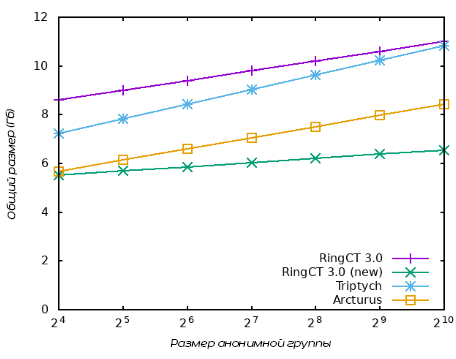
\includegraphics[width=0.6\textwidth]{size.png}
\caption{Общее увеличение размера блокчейна в зависимости от размера анонимной группы}
\label{fig:size}
\end{figure}

\begin{figure}
\centering
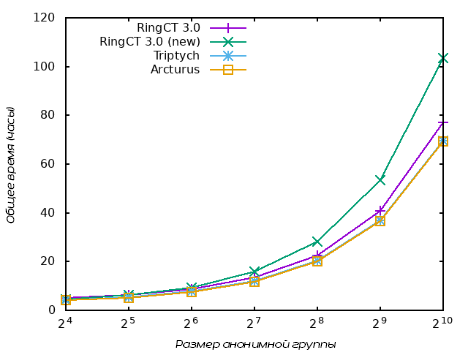
\includegraphics[width=0.6\textwidth]{time.png}
\caption{Общее время верификации в зависимости от размера анонимной группы}
\label{fig:time}
\end{figure}

Несмотря на то, что обновлённая версия протокола RingCT 3.0, представленная в работе \cite{rct3}, обеспечивает превосходное масштабирование, требование, согласно которому $w$ должно быть возведено во вторую степень (заполнено до этого значения), является причиной плохого масштабирования времени верификации.
В сравнении предлагаемая нами конструкция обеспечивает более низкую общую сложность верификации за счёт масштабирования общего размера.


\bibliographystyle{plain}
\bibliography{main}

\end{document}
